\documentclass[11pt,a4paper]{article}


%  Packages

\usepackage{amsmath,amssymb,amsthm}
\usepackage{mathtools}
\usepackage[T1]{fontenc}
\usepackage[utf8]{inputenc}
% microtype removed for compatibility
\usepackage{hyperref}
\usepackage{cleveref}
\usepackage{enumitem}
\usepackage{booktabs}
\usepackage{graphicx}
\usepackage{geometry}
\geometry{margin=2.5cm}


%  Theorem environments

\newtheorem{theorem}{Theorem}[section]
\newtheorem{proposition}[theorem]{Proposition}
\newtheorem{corollary}[theorem]{Corollary}
\newtheorem{lemma}[theorem]{Lemma}
\newtheorem{definition}[theorem]{Definition}
\newtheorem{remark}[theorem]{Remark}
\newtheorem{hypothesis}[theorem]{Hypothesis}


%  Macros

\newcommand{\Lproj}{\Lambda_{\mathrm{proj}}}
\newcommand{\nexit}{n_{\mathrm{exit}}}
\newcommand{\lpm}{\lambda_{\pm}}
\newcommand{\ltwo}{\lambda_{2}}
\newcommand{\hG}{h\!\left(G(n)\right)}
\newcommand{\EP}{E_{\mathrm{P}}}
\newcommand{\FKM}{F_{\mathrm{KM}}}
\newcommand{\rhoKM}{\rho_{\mathrm{KM}}}
\newcommand{\Mi}{M_i}
\newcommand{\Mj}{M_j}


\begin{document}

  \title{Projective Dynamics and Mass Hierarchy: Hierarchical Amplification via Growing Relational Valence}
  \author{J\'er\^ome Beau\\[4pt]
  \small Independent Researcher, Cosmochrony Project\\
  \small \texttt{contact@cosmochrony.org}
  }
  \date{March 2026}
  \maketitle


  \begin{abstract}
    The companion papers in the Admissibility Sub-Programme established two results:
    the representation-theoretic structure of ADE binary Cayley graphs fixes the number
    and ordering of stratigraphic levels~\cite{Beau2026a4}, and the projective resolution
    satisfies $\Lproj(n) \asymp \ltwo(n)$ under the isoperimetric closure
    hypothesis~\cite{Beau2026a5}.
    In the Lubotzky--Phillips--Sarnak (LPS) graph model at fixed prime~$p$,
    the algebraic connectivity $\ltwo(n)$ converges to a constant,
    making $\Lproj$ asymptotically static.
    This static regime produces mass ratios in~$[0.10,\,2.2]$,
    far below the $10^{-3}$--$10^{-5}$ range observed in the Standard Model,
    and inverts the mass ordering expected from the admissibility envelope.

    We show that both failures are resolved by allowing the effective
    relational valence $p$ to grow with the cascade rank~$n$.
    As $p(n)\to\infty$, the Kesten--McKay spectral support
    $[\lambda_{-}(p),\lambda_{+}(p)]$ narrows toward the midpoint~$\lambda=1$.
    The three fixed ADE eigenvalue levels exit the support in a rank-dependent
    order determined by their distance from~$1$: the level farthest from~$1$
    exits first and therefore stabilises at the highest mass.
    For the physically relevant ADE substrates this restores the admissibility ordering
    $M_{3}>M_{2}>M_{1}$ without additional tuning.
    The exit ranks satisfy an implicit equation
    $\lambda_{i} = \lambda_{+}(p(\nexit(\lambda_{i})))$,
    which for a power-law growth $p(n)\sim n^{\beta}$ yields
    mass ratios that grow rapidly with~$\beta$,
    providing a single falsifiable structural parameter.
  \end{abstract}

  \medskip
  \noindent\textbf{Keywords:}
  spectral graph theory; Ramanujan graphs; Kesten--McKay distribution;
  projective resolution; mass hierarchy; relational valence.

  \clearpage
  \tableofcontents

  \section{Introduction}
    \label{sec:intro}

    \subsection{Context and logical chain}
      \label{subsec:context}

      The Cosmochrony Bounded Admissibility framework~\cite{Cosmochrony}
      associates to each cascade rank~$n$ an energy scale $E_n = \EP/n$
      and a projective resolution $\Lproj(n)$: a spectral mode of eigenvalue~$\lambda$
      is admissible at rank~$n$ if and only if $\lambda \leq \Lproj(n)$.
      The stabilisation rank of a mode is the first~$n$ at which it ceases to be admissible,
      and the corresponding energy is the proxy for the physical mass of the associated
      particle sector.

      Four preceding papers in the Admissibility Sub-Programme have progressively
      constrained this picture.
      Step~1~\cite{Beau2026a1} established that the bounded-flux constraint
      selects spin-$\tfrac{1}{2}$ sectors as spectrally dominant on Cayley graphs of
      $\mathrm{SU}(2)$ subgroups.
      Step~2~\cite{Beau2026a2} identified the binary icosahedral group~$2I$ as the
      unique maximiser of the spectral capacity functional.
      Step~3~\cite{Beau2026a4} showed that exactly four pairs $(G,S)$ from the
      ADE binary groups produce Cayley graphs with exactly three distinct non-zero eigenvalues,
      yielding a three-level stratigraphic structure compatible with three fermion generations,
      and proved a no-go theorem ruling out scalar calibration as the source of level
      discreteness.
      Step~4~\cite{Beau2026a5} derived the isoperimetric law
      $\Lproj(n)\asymp h(G(n))^{2}$ and, under a spectral-isoperimetric saturation
      hypothesis, the linear law $\Lproj(n)\asymp\ltwo(n)$.
      It then evaluated the resulting mass ratios in the LPS model at fixed prime~$p$
      and identified both the ordering inversion and the amplitude failure as consequences
      of the asymptotic constancy of~$\Lproj$ in that regime.
      Step~5a~\cite{Beau2026a6} establishes, in a companion paper written concurrently
      with the present work, that allowing $p$ to grow with the cascade rank removes
      the fixed-valence saturation and restores the correct mass ordering
      $M_3 > M_1 > M_2$ through the support-narrowing mechanism.
      That paper explicitly leaves open the quantitative determination of the
      inter-generation mass ratios, which is the central result of the present paper.

      The present paper is Step~5 of the sub-programme.
      Its starting point is the open direction~(O1) identified in~\cite{Beau2026a5}:
      allow the effective relational valence~$p$ to grow with the cascade rank.

    \subsection{What the static LPS regime established and where it fails}
      \label{subsec:static-failure}

      In the LPS model with fixed prime~$p$, the algebraic connectivity satisfies
      \begin{equation}
        \ltwo(n) \;\longrightarrow\; \lambda_{2}^{*}(p)
        \;:=\; 1 - \frac{2\sqrt{p}}{p+1}
        \qquad (n\to\infty),
      \end{equation}
      so $\Lproj$ converges to a constant $\Lambda_{0}(p)$
      (Proposition~4.1 of~\cite{Beau2026a5}).
      In this static-threshold regime the only active ordering mechanism is the
      Kesten--McKay saturation condition $N(\lambda_{i};n)\geq k\dim\rho_{\lambda_i}$.
      The resulting mass formula is
      \begin{equation}
        \label{eq:static-mass}
        \frac{\Mi}{\Mj}
        \;=\;
        \frac{\FKM(\lambda_{i})}{\FKM(\lambda_{j})}
        \cdot
        \frac{\dim\rho_{\lambda_{j}}}{\dim\rho_{\lambda_{i}}},
      \end{equation}
      where $\FKM$ is the Kesten--McKay cumulative distribution function supported on
      $[\lambda_{-}(p),\lambda_{+}(p)]$ with $\lpm(p)= 1\mp 2\sqrt{p}/(p+1)$.

      As shown numerically in~\cite{Beau2026a5},
      equation~\eqref{eq:static-mass} produces ratios in~$[0.10,\,2.2]$
      for all admissible primes and all three-level ADE substrates,
      whereas the observed inter-generation mass ratios span
      $10^{-3}$--$10^{-5}$ for charged leptons and up-type quarks.
      Furthermore, the ratio $c_{3}/\dim\rho_{3}$ exceeds $c_{1}/\dim\rho_{1}$
      for the 2I (ord-4) substrate, inverting the ordering
      $M_{3}>M_{2}>M_{1}$ expected from the Born--Infeld admissibility envelope.

      Both failures have a common structural cause: the threshold~$\Lproj$ does not vary
      significantly along the cascade, so modes with spectrally similar eigenvalues are
      distinguished only by modest differences in~$\FKM$, which are of order unity.
      Generating the observed amplification requires a mechanism through which small
      spectral differences translate into large differences in stabilisation rank.

    \subsection{The dynamic degree of freedom: $p(n)\to\infty$}
      \label{subsec:dynamic-dof}

      The LPS construction at fixed prime~$p$ is only one point in a larger family.
      Physically, the prime~$p$ controls the effective relational valence of the substrate:
      the relaxation graph $G(n)$ is $(p+1)$-regular, so each relational node maintains
      $p+1$ active connections.
      A growing cascade need not maintain a fixed valence: as the number of active
      relational nodes increases, the connectivity structure of the substrate may become
      richer, corresponding to an effective increase of~$p$.

      Allowing $p$ to depend on the cascade rank~$n$ introduces a new dynamical degree
      of freedom that was held fixed in the analysis of~\cite{Beau2026a5}.
      Its key spectral consequence is a progressive narrowing of the Kesten--McKay support:
      \begin{equation}
        \lambda_{+}(p) - \lambda_{-}(p)
        \;=\; \frac{4\sqrt{p}}{p+1}
        \;\longrightarrow\; 0
        \qquad (p\to\infty).
      \end{equation}
      As the support shrinks toward~$\{\lambda=1\}$, the three fixed ADE eigenvalue levels
      $\lambda_{1}<\lambda_{2}<\lambda_{3}$ eventually exit the support.
      The exit occurs in an order determined entirely by the distance of each level from
      the midpoint~$1$: the level with the largest distance exits first.
      Since $\lambda_{3}>1$ and for the relevant ADE substrates $\lambda_{3}-1 > 1-\lambda_{1}$,
      the level~$\lambda_{3}$ exits before~$\lambda_{1}$,
      yielding stabilisation ranks $\nexit(\lambda_{3}) < \nexit(\lambda_{1})$
      and therefore masses $M_{3}>M_{1}$,
      in agreement with the admissibility ordering.

      This mechanism, which we call \emph{support-narrowing amplification}, is the
      central object of the present paper.
      It does not introduce free parameters beyond the growth law $p(n)$,
      and the resulting mass ratios are sharply sensitive to the exponent governing
      that growth, providing a falsifiable structural prediction.

    \subsection{Structure of the paper}
      \label{subsec:structure}

      Section~\ref{sec:nogo} collects the relevant results of~\cite{Beau2026a5}
      concerning the static LPS regime and states both failures precisely, serving as
      the logical starting point for the dynamic extension.
      Section~\ref{sec:dynamic} introduces the dynamic valence hypothesis
      $p = p(n)$ and derives the support-narrowing mechanism.
      Section~\ref{sec:exit} formalises the exit-rank equation and derives the
      resulting mass formula.
      Section~\ref{sec:massformula} evaluates mass ratios for power-law
      growth $p(n)\sim n^{\beta}$ and compares with Standard Model data.
      Section~\ref{sec:ADE} discusses the compatibility of the dynamic mechanism
      with the three-level ADE structure established in~\cite{Beau2026a4}.
      Section~\ref{sec:numerical} provides a numerical illustration.
      Section~\ref{sec:architecture} places O3 in the global O-series architecture.
      Section~\ref{sec:falsifiability} discusses the falsifiable predictions.
      Section~\ref{sec:conclusion} concludes.

  \section{The Static LPS No-Go: Precise Statement}
    \label{sec:nogo}


    This section assembles the results of~\cite{Beau2026a5} that will serve as
    the logical departure point for the dynamic extension.
    No new results are proved here; the purpose is to state the two failures of the
    static regime with the precision required to identify their structural cause.

    \subsection{Setup and notation}
      \label{subsec:setup}

      Throughout this paper, $n\in\mathbb{N}_{>0}$ denotes the \emph{cascade rank},
      an integer-valued depth parameter indexing successive stages of the
      Cosmochrony relaxation cascade.
      The energy available at rank~$n$ is $E_{n} = \EP/n$, where $\EP$ is the Planck energy.
      We write $G(n)$ for the effective relaxation graph at rank~$n$: a connected,
      $d(n)$-regular, undirected graph.
      Its normalised Laplacian is $L_{G(n)}$, with eigenvalues
      $0 = \mu_{0} < \mu_{1} \leq \mu_{2} \leq \cdots$.
      The \emph{algebraic connectivity} (Fiedler value) is $\ltwo(n) := \mu_{1}(L_{G(n)})$.

      The projective resolution is
      \begin{equation}
        \label{eq:Lproj-def}
        \Lproj(n)
        \;=\;
        \frac{c_{\mathrm{BI}}(n)^{2}}{A_{\min}^{2}},
      \end{equation}
      where $c_{\mathrm{BI}}(n)>0$ is the global projective flux bound and $A_{\min}>0$
      is a fixed scale independent of~$n$.
      Under the isoperimetric closure hypothesis (Hypothesis~2.1
      of~\cite{Beau2026a5}), $c_{\mathrm{BI}}(n)\asymp\hG$, giving
      $\Lproj(n)\asymp h(G(n))^{2}$.
      Under the additional spectral-isoperimetric saturation hypothesis (Hypothesis~2.2
      of~\cite{Beau2026a5}), the linear law
      \begin{equation}
        \label{eq:linear-law}
        \Lproj(n) \;\asymp\; \ltwo(n)
      \end{equation}
      holds with constants independent of~$n$.

      The LPS graph $X^{p,q}$ is a $(p+1)$-regular Ramanujan graph on
      $\mathrm{PSL}(2,\mathbb{F}_{q})$, with $|V(X^{p,q})| = \tfrac{1}{2}q(q^{2}-1)$.
      The physical identification $n\sim|V(G(n))|$ gives $n\sim q^{3}/2$,
      so $q\sim(2n)^{1/3}$.
      The Ramanujan property gives the uniform lower bound
      \begin{equation}
        \label{eq:ramanujan}
        \ltwo\!\left(X^{p,q}\right)
        \;\geq\;
        1 - \frac{2\sqrt{p}}{p+1}
        \qquad \text{for all admissible } q.
      \end{equation}

    \subsection{Asymptotic constancy of the projective threshold}
      \label{subsec:asymptotic-constancy}

      The following result is Proposition~4.1 of~\cite{Beau2026a5}.

      \begin{proposition}[Asymptotic constancy of $\Lproj$, {\cite{SpectralRelaxation}}]
        \label{prop:static}
        Let $p$ be a fixed prime.
        Under the linear law~\eqref{eq:linear-law}, the projective resolution satisfies
        \begin{equation}
          \Lproj(n) \;\longrightarrow\; \Lambda_{0}(p)
          \;:=\; \frac{C\,\lambda_{2}^{*}(p)}{A_{\min}^{2}},
          \qquad
          \lambda_{2}^{*}(p) = 1 - \frac{2\sqrt{p}}{p+1},
          \qquad
          (n\to\infty),
        \end{equation}
        where $C>0$ absorbs the implicit constant in~\eqref{eq:linear-law}.
        In particular, $\Lproj$ is asymptotically static: its variation along the
        cascade is suppressed as $n^{-1/3}$.
      \end{proposition}

      When $\Lproj$ is asymptotically constant, the support condition
      $\lambda_{i}\leq\Lproj(n)$ reduces to a fixed constraint for all sufficiently
      large~$n$, and the sole ordering mechanism becomes the saturation condition
      $N(\lambda_{i};n)\geq k\dim\rho_{\lambda_{i}}$.

    \subsection{The Kesten--McKay mass formula and its two failures}
      \label{subsec:km-failures}

      For the three-level ADE substrates identified in~\cite{Beau2026a4},
      the Kesten--McKay cumulative distribution function
      $\FKM(\lambda) = \mu^{(p)}_{\mathrm{KM}}((-\infty,\lambda])$
      controls the linear growth of the spectral counting function:
      $N(\lambda;n)\sim \FKM(\lambda)\cdot n$ as $n\to\infty$
      (Proposition~4.2 of~\cite{Beau2026a5}).
      The stabilisation rank is therefore
      $n_{\mathrm{proj}}(\lambda_{i})\sim k\dim\rho_{\lambda_{i}}/\FKM(\lambda_{i})$,
      giving the mass formula~\eqref{eq:static-mass}.

      Two structural failures of this formula are established
      in Section~5 of~\cite{Beau2026a5}.

      \begin{proposition}[Amplitude failure]
        \label{prop:amplitude}
        For all three three-level ADE substrates and all admissible primes,
        the predicted mass ratios satisfy
        \begin{equation}
          0.10 \;\leq\; \frac{\Mi}{\Mj} \;\leq\; 2.2.
        \end{equation}
        The observed inter-generation ratios for charged leptons
        ($m_{e}/m_{\tau}\approx 2.9\times10^{-4}$)
        and up-type quarks ($m_{u}/m_{t}\sim10^{-5}$)
        fall short of the predicted range by two to four orders of magnitude.
      \end{proposition}

      \begin{proposition}[Ordering failure for $2I$ (ord-4)]
        \label{prop:ordering}
        For the $2I$ substrate with order-4 generators,
        the ratio $c_{3}(p)/\dim\rho_{3}$ exceeds $c_{1}(p)/\dim\rho_{1}$
        for all admissible primes $p\leq 29$,
        predicting $M_{1}<M_{3}$ in contradiction with
        the admissibility ordering $M_{1}>M_{3}$
        (lower eigenvalue $\Leftrightarrow$ wider admissibility window
        $\Leftrightarrow$ heavier particle) established in~\cite{Beau2026a4}.
      \end{proposition}

      \begin{remark}[Common structural cause]
        \label{rem:common-cause}
        Both failures share the same structural origin.
        In the static-threshold regime, all three ADE levels simultaneously satisfy
        the support condition $\lambda_{i}\leq\Lambda_{0}(p)$ for all sufficiently large~$n$.
        Level discrimination therefore relies entirely on differences in~$\FKM(\lambda_{i})$,
        which are of order unity by the boundedness of~$\FKM$.
        No amount of tuning within the static LPS model can produce ratios
        outside~$[0.1,2.2]$ or repair the ordering, because both are consequences
        of~$\FKM$ being a fixed bounded function independent of~$n$.
        The only resolution is to make the support condition itself $n$-dependent,
        which requires $\Lproj(n)$ to vary non-trivially along the cascade.
      \end{remark}

    \subsection{Why varying $p$ is the natural resolution}
      \label{subsec:why-p}

      Remark~\ref{rem:common-cause} identifies the precise structural requirement:
      the support of the Kesten--McKay measure must shrink as~$n$ grows,
      so that the ADE levels $\lambda_{1}<\lambda_{2}<\lambda_{3}$ exit the support
      at different cascade ranks.
      The Kesten--McKay support is $[\lambda_{-}(p),\lambda_{+}(p)]$
      with $\lpm(p) = 1\mp 2\sqrt{p}/(p+1)$, so the support width
      $\lambda_{+}-\lambda_{-} = 4\sqrt{p}/(p+1)$ is a strictly decreasing function of~$p$.
      The only free structural parameter that controls this width is~$p$.

      This observation, noted qualitatively in direction~(O1) of~\cite{Beau2026a5}
      (cf.\ Figure~3 therein), motivates the central hypothesis of the present paper:
      the effective prime governing the relaxation graph grows with the cascade rank.
      Section~\ref{sec:dynamic} formalises this hypothesis and derives its consequences.

      The support-narrowing mechanism introduced here was identified concurrently
      and independently in~\cite{Beau2026a6}, which proves the exit ordering
      as a formal theorem.
      The present paper takes the mechanism as established and focuses on
      the quantitative consequences: the power-law growth ansatz $p(n)\sim n^\beta$,
      the explicit mass formula~\eqref{eq:mass-ratio-powerlaw}, and the
      compatibility window $\beta^{*}\in(0.09,\,0.13)$ matching the charged-lepton sector.

  \section{Growing Relational Valence: the Dynamic Hypothesis}
    \label{sec:dynamic}

    \subsection{Physical motivation}
      \label{subsec:motivation}

      In the LPS construction, the prime $p$ determines the degree $d = p+1$ of the
      relaxation graph: each relational node maintains exactly $p+1$ active connections.
      The analysis of Section~\ref{sec:nogo} treated $p$ as a fixed structural constant,
      independent of the cascade rank~$n$.
      This assumption is physically restrictive.
      Along the relaxation cascade, the number of active relational nodes grows with~$n$,
      and there is no \textit{a priori} reason why the local connectivity of the
      substrate should remain frozen as the global structure becomes richer.
      On the contrary, the Cosmochrony picture of an evolving relational
      substrate~\cite{Cosmochrony} suggests that increasing cascade depth corresponds
      to increasing relational accessibility: more nodes become mutually reachable,
      and the effective valence of the graph~-- the number of distinct relational
      connections each node can sustain~-- grows accordingly.

      We formalise this observation as the central structural hypothesis of this paper.

      \begin{hypothesis}[Dynamic valence growth]
        \label{hyp:dynamic-p}
        The effective prime governing the LPS relaxation graph at cascade rank~$n$
        is a non-decreasing function $p\colon \mathbb{N}_{>0} \to \mathcal{P}$,
        where $\mathcal{P}$ denotes the set of odd primes congruent to $1\pmod{4}$,
        satisfying $p(n) \to \infty$ as $n \to \infty$.
        The relaxation graph at rank~$n$ is the LPS graph $X^{p(n),q(n)}$,
        with $q(n)$ determined by the identification $n \sim \tfrac{1}{2}q(n)(q(n)^2 - 1)$.
      \end{hypothesis}

      \begin{remark}[Status of Hypothesis~\ref{hyp:dynamic-p}]
        \label{rem:status-hyp}
        Hypothesis~\ref{hyp:dynamic-p} is a structural postulate.
        It extends the isoperimetric closure hypothesis of~\cite{Beau2026a5}
        by promoting the previously fixed parameter~$p$ to a dynamical variable.
        A derivation of the specific growth law $p(n)$ from the internal
        dynamics of the Cosmochrony substrate remains an open problem
        and is discussed in Section~\ref{sec:falsifiability}.
        The present paper establishes the consequences of
        Hypothesis~\ref{hyp:dynamic-p} for the mass hierarchy,
        independently of the precise growth law.
      \end{remark}

    \subsection{Spectral consequence: support narrowing}
      \label{subsec:narrowing}

      The key spectral effect of $p(n)\to\infty$ is a progressive contraction
      of the Kesten--McKay support.
      Recall that the support of $\mu^{(p)}_{\mathrm{KM}}$ is the interval
      $[\lambda_{-}(p),\lambda_{+}(p)]$ with
      \begin{equation}
        \label{eq:support-edges}
        \lambda_{\pm}(p) \;=\; 1 \mp \frac{2\sqrt{p}}{p+1}.
      \end{equation}
      The support width satisfies
      \begin{equation}
        \label{eq:support-width}
        \lambda_{+}(p) - \lambda_{-}(p)
        \;=\; \frac{4\sqrt{p}}{p+1}
        \;\sim\; \frac{4}{\sqrt{p}}
        \qquad (p \to \infty),
      \end{equation}
      which tends to zero monotonically.
      In the limit $p\to\infty$, the Kesten--McKay measure converges weakly to
      the Dirac mass at $\lambda = 1$, consistent with the fact that
      the spectral measure of the $S^3$ Laplacian is recovered in that
      limit~\cite{Beau2026a5}.

      \begin{proposition}[Support narrowing]
        \label{prop:narrowing}
        Under Hypothesis~\ref{hyp:dynamic-p}, for any fixed $\lambda \neq 1$,
        there exists a finite rank $\nexit(\lambda) \in \mathbb{N}_{>0}$ such that
        \begin{equation}
          \label{eq:exit-condition}
          \lambda \;\notin\; \bigl[\lambda_{-}(p(n)),\;\lambda_{+}(p(n))\bigr]
          \qquad \text{for all } n \geq \nexit(\lambda).
        \end{equation}
        Equivalently, $\nexit(\lambda)$ is the first rank at which the effective
        Kesten--McKay support no longer contains~$\lambda$.
      \end{proposition}

      \begin{proof}
        Since $\lambda_{+}(p) - \lambda_{-}(p) \to 0$ by~\eqref{eq:support-width}
        and $p(n)\to\infty$ by Hypothesis~\ref{hyp:dynamic-p},
        for any $\lambda \neq 1$ there exists $p^{*}$ such that
        $|\lambda - 1| > 2\sqrt{p^{*}}/(p^{*}+1)$.
        Since $p(n)\to\infty$, there exists $\nexit(\lambda)$ such that
        $p(n) \geq p^{*}$ for all $n \geq \nexit(\lambda)$,
        whence $\lambda \notin [\lambda_{-}(p(n)),\lambda_{+}(p(n))]$.
      \end{proof}

      \begin{remark}[Explicit exit rank for power-law growth]
        \label{rem:exit-explicit}
        When $p(n) \sim A n^{\beta}$ for constants $A > 0$ and $\beta > 0$,
        the exit condition $\lambda_{+}(p(\nexit)) = \lambda$
        (for $\lambda > 1$; symmetrically for $\lambda < 1$) reads
        \begin{equation}
          \label{eq:exit-implicit}
          \lambda \;=\; 1 + \frac{2\sqrt{p(\nexit)}}{p(\nexit)+1}.
        \end{equation}
        Inverting to leading order in large~$p$:
        $p(\nexit) \approx 4(\lambda-1)^{-2}$, and hence
        \begin{equation}
          \label{eq:exit-rank}
          \nexit(\lambda) \;\approx\;
          \left(\frac{4}{A\,(\lambda-1)^{2}}\right)^{1/\beta}.
        \end{equation}
        The exit rank is therefore a strictly decreasing function of $|\lambda - 1|$:
        levels farther from the midpoint~$1$ exit the support at smaller rank.
      \end{remark}

    \subsection{Exit ordering and restored mass hierarchy}
      \label{subsec:ordering}

      The three ADE eigenvalue levels $\lambda_1 < \lambda_2 < \lambda_3$
      are fixed properties of the chosen ADE substrate $(G,S)$,
      independent of the cascade dynamics.
      The support-narrowing mechanism assigns to each level a finite exit
      rank $\nexit(\lambda_i)$, and the ordering of these ranks determines
      the mass ordering.

      \begin{proposition}[Exit ordering]
        \label{prop:exit-ordering}
        Let $\lambda_1 < 1 < \lambda_3$ be the lowest and highest ADE eigenvalue
        levels with $|\lambda_3 - 1| > |\lambda_1 - 1| > 0$.
        Under Hypothesis~\ref{hyp:dynamic-p}, the exit ranks satisfy
        \begin{equation}
          \label{eq:exit-ordering}
          \nexit(\lambda_3) \;<\; \nexit(\lambda_1) \;<\; \nexit(\lambda_2) = +\infty.
        \end{equation}
      \end{proposition}

      \begin{proof}
        By Remark~\ref{rem:exit-explicit}, $\nexit(\lambda)$ is strictly decreasing
        in $|\lambda - 1|$.
        Since $|\lambda_3 - 1| > |\lambda_1 - 1| > 0$,
        one has $\nexit(\lambda_3) < \nexit(\lambda_1) < +\infty$.
        The midpoint level $\lambda_2 = 1$ is the centre of symmetry of the
        Kesten--McKay support for all~$p$, so
        $\lambda_2 \in [\lambda_{-}(p),\lambda_{+}(p)]$ for every prime~$p$,
        giving $\nexit(\lambda_2) = +\infty$.
      \end{proof}

      \begin{remark}[Verification for the physically relevant substrates]
        \label{rem:asymmetry}
        The asymmetry condition $|\lambda_3 - 1| > |\lambda_1 - 1|$ is
        satisfied by both physically relevant ADE substrates:
        \begin{itemize}[nosep]
    \item $2I$, ord-4 generators: $\lambda_1 = 4/5$, $\lambda_3 = 4/3$,
    giving $|\lambda_3 - 1| = 1/3 > |\lambda_1 - 1| = 1/5$.\quad\checkmark
    \item $2I$, ord-5 generators: $\lambda_1 = 5/6$, $\lambda_3 = 5/4$,
    giving $|\lambda_3 - 1| = 1/4 > |\lambda_1 - 1| = 1/6$.\quad\checkmark
        \end{itemize}
        This is a structural property of the ADE representation spectrum,
        not an additional hypothesis.
      \end{remark}

    \subsection{From exit ranks to physical masses}
      \label{subsec:mass-interpretation}

      A mode at ADE level $\lambda_i$ that exits the Kesten--McKay support at
      rank $\nexit(\lambda_i)$ is no longer admissible for $n \geq \nexit(\lambda_i)$.
      Its stabilisation rank is therefore $n_{\mathrm{proj}}(\lambda_i) = \nexit(\lambda_i)$,
      and the corresponding stabilisation mass is
      \begin{equation}
        \label{eq:mass-exit}
        M_i \;\propto\; \frac{\EP}{\nexit(\lambda_i)}.
      \end{equation}
      The ordering~\eqref{eq:exit-ordering} immediately gives
      $M_3 > M_1 > M_2$,
      restoring the hierarchy expected from the admissibility
      envelope of~\cite{Beau2026a4} and resolving the ordering failure
      of Proposition~\ref{prop:ordering} without any tuning.

      The inter-generation mass ratio is
      \begin{equation}
        \label{eq:mass-ratio-exit}
        \frac{M_i}{M_j}
        \;=\; \frac{\nexit(\lambda_j)}{\nexit(\lambda_i)}.
      \end{equation}
      For power-law growth $p(n) \sim A n^{\beta}$,
      substituting~\eqref{eq:exit-rank} gives
      \begin{equation}
        \label{eq:mass-ratio-powerlaw}
        \frac{M_i}{M_j}
        \;\approx\;
        \left(\frac{|\lambda_i - 1|}{|\lambda_j - 1|}\right)^{2/\beta},
        \qquad i < j.
      \end{equation}
      This is the central quantitative prediction of the paper.
      The amplification exponent $2/\beta$ converts spectral ratios of order~$2$
      (the typical ratio $|\lambda_i-1|/|\lambda_j-1|$ for the ADE substrates)
      into mass ratios that grow without bound as $\beta \to 0$.

    \subsection{Parametrisation of $p(n)$ and structural scope}
      \label{subsec:parametrisation}

      Two natural parametrisations span the physically relevant range:
      \begin{align}
        \label{eq:power-law}
        p(n) \;&\sim\; A\, n^{\beta},
        \qquad A > 0,\; \beta > 0
        \qquad \text{(power-law growth)},\\[4pt]
        \label{eq:log-growth}
        p(n) \;&\sim\; B\, \log n,
        \qquad B > 0
        \qquad \text{(logarithmic growth)}.
      \end{align}
      Power-law growth~\eqref{eq:power-law} is the canonical choice:
      it introduces a single dimensionless exponent~$\beta$ as the structural
      parameter controlling the amplification, and the mass
      formula~\eqref{eq:mass-ratio-powerlaw} depends on~$\beta$ alone
      (the prefactor~$A$ cancels in ratios).
      Logarithmic growth~\eqref{eq:log-growth} is the limiting case $\beta \to 0^{+}$
      and would produce exit ranks growing faster than any power, hence larger
      amplification for a given spectral asymmetry; it is discussed as a boundary
      case in Section~\ref{sec:falsifiability}.

      The present paper focuses on power-law growth as the minimal
      one-parameter family capturing the amplification mechanism.
      The exponent~$\beta$ is not a free fitting parameter in the usual sense:
      it characterises the rate of growth of relational accessibility along the cascade,
      a structural property of the substrate that in principle admits an independent
      derivation within the Cosmochrony framework, as discussed in
      Section~\ref{sec:falsifiability}.

  \section{Mass Ratios from Dynamic Valence Growth}
    \label{sec:massformula}

    \subsection{Exit-rank formula under power-law growth}
      \label{subsec:exit-formula}

      We now evaluate the mass ratios implied by the support-narrowing mechanism
      of Section~\ref{sec:dynamic}.
      Under the power-law ansatz $p(n) \sim A n^{\beta}$ ($A>0$, $\beta>0$),
      the implicit exit condition~\eqref{eq:exit-implicit} reduces at leading order to
      \begin{equation}
        \label{eq:pexit-leading}
        p_{\mathrm{exit}}(\lambda_i)
        \;\approx\; \frac{4}{(\lambda_i - 1)^2},
        \qquad |\lambda_i - 1| \ll 1,
      \end{equation}
      and the exit rank is therefore
      \begin{equation}
        \label{eq:nexit-powerlaw}
        \nexit(\lambda_i)
        \;\approx\; \left(\frac{4}{A\,(\lambda_i-1)^2}\right)^{1/\beta}.
      \end{equation}
      Since $M_i \propto \EP/\nexit(\lambda_i)$ by~\eqref{eq:mass-exit},
      the inter-generation mass ratio reads
      \begin{equation}
        \label{eq:ratio-beta}
        \frac{M_i}{M_j}
        \;\approx\;
        \left(\frac{|\lambda_i - 1|}{|\lambda_j - 1|}\right)^{2/\beta},
        \qquad i < j.
      \end{equation}
      The prefactor $A$ cancels in all ratios.
      The exponent $2/\beta$ is the sole amplification parameter:
      small spectral distances $|\lambda_i - 1|$ are raised to the power $2/\beta$,
      converting spectral asymmetries of order unity into mass ratios of arbitrary
      magnitude as $\beta \to 0^{+}$.

    \subsection{Spectral input: exact eigenvalues of the ADE substrates}
      \label{subsec:spectral-input}

      The two physically relevant substrates identified in~\cite{Beau2026a4}
      carry the following normalised Laplacian eigenvalues.
      All eigenvalues are expressed in the normalised convention
      $\lambda_i^{\mathrm{norm}} = \lambda_i^{\mathrm{raw}}/|S|$,
      where $|S|$ is the size of the generating set (equivalently the degree
      of the Cayley graph), consistent with the normalised Laplacian
      $L = I - A/d$ used for the LPS graphs in~\cite{Beau2026a5}.
      The ratios $|\lambda_i - 1|/|\lambda_j - 1|$ entering the mass
      formula~\eqref{eq:ratio-beta} are invariant under any uniform
      rescaling of the spectrum that preserves the midpoint $\lambda = 1$,
      providing a further robustness check.

      \medskip
      \noindent
      \textbf{$2I$, order-4 generators} ($|S| = 30$, raw eigenvalues $\{24, 30, 40\}$):
      \begin{equation}
        \label{eq:evals-ord4}
        \lambda_1 = \tfrac{4}{5},
        \qquad
        \lambda_2 = 1,
        \qquad
        \lambda_3 = \tfrac{4}{3}.
      \end{equation}
      The distances to the midpoint are
      $d_1 := |\lambda_1 - 1| = \tfrac{1}{5}$ and
      $d_3 := |\lambda_3 - 1| = \tfrac{1}{3}$,
      giving $d_1/d_3 = \tfrac{3}{5}$.

      \medskip
      \noindent
      \textbf{$2I$, order-5 generators} ($|S| = 24$, raw eigenvalues $\{20, 24, 30\}$):
      \begin{equation}
        \label{eq:evals-ord5}
        \lambda_1 = \tfrac{5}{6},
        \qquad
        \lambda_2 = 1,
        \qquad
        \lambda_3 = \tfrac{5}{4}.
      \end{equation}
      The distances are
      $d_1 = \tfrac{1}{6}$ and $d_3 = \tfrac{1}{4}$,
      giving $d_1/d_3 = \tfrac{2}{3}$.

      \medskip
      \noindent
      In both cases $\lambda_2 = 1$ exactly, so $\nexit(\lambda_2) = +\infty$
      and the support-narrowing mechanism assigns no finite exit rank to the
      second generation.\footnote{%
    The absence of a support-exit rank for $\lambda_2 = 1$ does not imply
    a vanishing physical mass.
    It reflects the structural fact that the level $\lambda_2 = 1$ lies
    permanently inside the Kesten--McKay support for all~$p$ and therefore
    requires a different stabilisation mechanism.
    The second-generation mass is determined by the KM saturation condition
    $N(\lambda_2; n) \geq k \dim\rho_{\lambda_2}$ of~\cite{Beau2026a5},
    which produces a finite stabilisation rank through spectral counting
    rather than support exit.
  }
      The second-generation mass requires the KM saturation mechanism
      of~\cite{Beau2026a5} to be assigned a finite value
      and is not the primary target of the present calculation.
      The central observable is the ratio $M_1/M_3$.

    \subsection{Scaling of mass ratios with $\beta$}
      \label{subsec:scaling}

      Substituting the spectral inputs~\eqref{eq:evals-ord4}--\eqref{eq:evals-ord5}
      into~\eqref{eq:ratio-beta} gives:
      \begin{align}
        \label{eq:ratio-ord4}
        \frac{M_1}{M_3}\bigg|_{2I,\,\mathrm{ord\text{-}4}}
        &\;\approx\; \left(\tfrac{3}{5}\right)^{2/\beta},\\[6pt]
        \label{eq:ratio-ord5}
        \frac{M_1}{M_3}\bigg|_{2I,\,\mathrm{ord\text{-}5}}
        &\;\approx\; \left(\tfrac{2}{3}\right)^{2/\beta}.
      \end{align}
      Table~\ref{tab:ratios} reports the predicted $M_1/M_3$ for selected values
      of~$\beta$, together with the observed charged-lepton ratio
      $m_e/m_\tau \approx 2.88 \times 10^{-4}$.

      \begin{table}[ht]
        \centering
        \caption{%
          Predicted mass ratio $M_1/M_3$ as a function of the growth exponent~$\beta$,
          for the two physically relevant ADE substrates.
          The observed value for charged leptons is
          $m_e/m_\tau \approx 2.88 \times 10^{-4}$.%
        }
        \label{tab:ratios}
        \smallskip
        \begin{tabular}{ccc}
          \toprule
          $\beta$ &
          $M_1/M_3$\ ($2I$ ord-4, $d_1/d_3 = 3/5$) &
          $M_1/M_3$\ ($2I$ ord-5, $d_1/d_3 = 2/3$) \\
          \midrule
          $0.05$ & $1.3 \times 10^{-9}$ & $9.0 \times 10^{-8}$ \\
          $0.10$ & $3.7 \times 10^{-5}$ & $3.0 \times 10^{-4}$ \\
          $0.13$ & $2.9 \times 10^{-4}$ & $\sim 10^{-3}$       \\
          $0.20$ & $6.0 \times 10^{-3}$ & $1.7 \times 10^{-2}$ \\
          $0.30$ & $3.3 \times 10^{-2}$ & $6.7 \times 10^{-2}$ \\
          $0.50$ & $1.3 \times 10^{-1}$ & $2.0 \times 10^{-1}$ \\
          $1.00$ & $3.6 \times 10^{-1}$ & $4.4 \times 10^{-1}$ \\
          \bottomrule
        \end{tabular}
      \end{table}

      \begin{remark}[Large and moderate $\beta$]
        \label{rem:large-beta}
        For $\beta \geq 1$, both substrates produce $M_1/M_3 > 0.3$,
        consistent with the static LPS range $[0.10, 2.2]$ of
        Proposition~\ref{prop:amplitude}.
        The dynamic mechanism recovers and continuously extends the static regime
        as $\beta$ decreases from unity toward zero.
        There is no discontinuity: the static regime corresponds to the
        limiting case where $p(n)$ grows slowly enough that
        the Kesten--McKay saturation condition dominates before
        the support exits the ADE levels.
      \end{remark}

    \subsection{Compatibility window for the charged leptons}
      \label{subsec:window}

      The observed charged-lepton ratios (PDG~2024) are
      \begin{equation}
        \label{eq:lepton-ratios}
        \frac{m_e}{m_\mu} \approx 4.84 \times 10^{-3},
        \qquad
        \frac{m_\mu}{m_\tau} \approx 5.95 \times 10^{-2},
        \qquad
        \frac{m_e}{m_\tau} \approx 2.88 \times 10^{-4}.
      \end{equation}
      The ratio $M_1/M_3$ in~\eqref{eq:ratio-beta} is the analogue of $m_e/m_\tau$
      (lowest-to-highest generation under the ordering of
      Proposition~\ref{prop:exit-ordering}).
      Matching $M_1/M_3 = m_e/m_\tau$ requires
      \begin{equation}
        \label{eq:beta-match}
        \frac{2}{\beta}\,\log\!\left(\frac{d_1}{d_3}\right)
        = \log\!\left(\frac{m_e}{m_\tau}\right).
      \end{equation}
      Solving for $\beta$ gives
      \begin{equation}
        \label{eq:beta-window}
        \beta^* \;=\;
        \frac{2\,\log(d_1/d_3)}{\log(m_e/m_\tau)}
        \;\approx\;
        \begin{cases}
          0.125 & \text{($2I$ ord-4, $d_1/d_3 = 3/5$),}\\[4pt]
          0.100 & \text{($2I$ ord-5, $d_1/d_3 = 2/3$).}
        \end{cases}
      \end{equation}
      Both values lie in the interval $\beta^{*} \in (0.09,\, 0.13)$,
      a narrow compatibility window determined entirely by the spectral structure
      of the ADE substrate and the observed lepton masses.

      \begin{remark}[Internal consistency: the two-ratio test]
        \label{rem:two-ratio}
        Equation~\eqref{eq:ratio-beta} predicts a single exponent~$\beta$ governing
        all three lepton ratios simultaneously, since only two levels ($\lambda_1$
        and $\lambda_3$) contribute exit ranks.
        For $2I$ (ord-4) with $\beta^{*} \approx 0.125$:
        \begin{equation}
          \frac{M_1}{M_3} = \left(\tfrac{3}{5}\right)^{16}
          \approx 2.8 \times 10^{-4}
          \qquad \text{vs.\ observed } m_e/m_\tau \approx 2.9 \times 10^{-4}.
        \end{equation}
        The ratio $M_1/M_2$ requires the KM saturation mechanism for $\lambda_2 = 1$
        and is not predicted by the exit formula alone.
        A self-consistent treatment of the intermediate generation
        is deferred to Section~\ref{sec:ADE}.
      \end{remark}

    \subsection{Physical interpretation}
      \label{subsec:interpretation}

      Equation~\eqref{eq:ratio-beta} encodes a structural amplification mechanism
      with three notable properties.

      First, the spectral ratios $d_i/d_j$ entering~\eqref{eq:ratio-beta}
      are of order $2/3$ to $3/5$ for both ADE substrates~-- modest asymmetries
      of order 50\%.
      The exponent $2/\beta^{*} \approx 16$ converts these into mass ratios spanning
      three and a half decades, without invoking any large dimensionless
      parameter in the Lagrangian.

      Second, the prefactor $A$ in $p(n) \sim A n^{\beta}$ plays no role in
      mass ratios: it cancels identically in~\eqref{eq:ratio-beta}.
      The sole structural parameter is the growth exponent~$\beta$.

      Third, the mechanism is discontinuous in the static limit.
      Setting $p(n) = p_0$ (constant) is not the limit $\beta \to 0$
      of power-law growth: it is a different functional form in which
      $\lambda_2(n)\to\lambda_2^*(p_0) < 1$ for all $n$,
      and the support never narrows.
      The two regimes~-- static and dynamic~-- are separated by a qualitative
      change in the long-run behaviour of the relaxation graph,
      not merely by a quantitative parameter limit.

  \section{Compatibility with ADE Spectral Structure}
    \label{sec:ADE}

    \subsection{Structural invariance of ADE eigenvalues}
      \label{subsec:ADE-invariance}

      The ADE eigenvalue levels $\lambda_1, \lambda_2, \lambda_3$ established
      in~\cite{Beau2026a4} are properties of the Cayley graph
      $\mathrm{Cay}(G, S)$ of the ADE binary group~$G$ with generating set~$S$.
      They are determined by the character sums
      \begin{equation}
        \label{eq:char-sum}
        \mu_{\rho}
        \;=\; \frac{1}{d_{\rho}} \sum_{s \in S} \chi_{\rho}(s),
      \end{equation}
      where $\rho$ ranges over the non-trivial irreducible representations of~$G$.
      The three distinct values taken by $\mu_\rho$ define the three levels;
      their exact rational values are~\eqref{eq:evals-ord4}--\eqref{eq:evals-ord5}.

      These eigenvalues depend only on $(G, S)$.
      They do not depend on the LPS prime~$p$, on the cascade rank~$n$,
      or on any property of the ambient relaxation graph $G(n) = X^{p(n), q(n)}$.
      The ADE eigenvalues are not approximations of the LPS spectrum;
      they are independent spectral data, upon which the LPS Kesten--McKay
      support acts as an external constraint.
      The dynamic valence hypothesis (Hypothesis~\ref{hyp:dynamic-p}) modifies
      the relaxation graph but leaves the ADE Cayley graph unchanged.
      The levels $\lambda_1, \lambda_2, \lambda_3$ are therefore invariant
      under the entire family of dynamics considered in this paper.

    \subsection{Separation between spectral support and intrinsic modes}
      \label{subsec:separation}

      Two distinct spectral objects must not be conflated:
      \begin{enumerate}[label=(\roman*), nosep]
  \item the \emph{Kesten--McKay spectral support} $[\lambda_{-}(p(n)),\lambda_{+}(p(n))]$,
  which is a property of the LPS relaxation graph $X^{p(n),q(n)}$
  and contracts as $p(n)\to\infty$;
  \item the \emph{ADE eigenvalue levels} $\{\lambda_1, \lambda_2, \lambda_3\}$,
  which are properties of the ADE Cayley graph
  and are independent of~$p(n)$.
      \end{enumerate}
      The support-narrowing mechanism acts entirely on object~(i).
      A mode at ADE level~$\lambda_i$ stabilises when $\lambda_i$ exits the
      support, i.e.\ when the ambient relaxation graph can no longer sustain
      propagation at that frequency.
      This is an extrinsic condition imposed on the modes by the relaxation environment;
      it does not alter the intrinsic eigenvalue of the mode.

      A potential objection is that changing $p(n)$ changes the LPS graphs,
      and hence changes the eigenstructure of the full substrate.
      This is correct at the level of the relaxation graph $G(n)$,
      whose eigenvalues do shift as $p$ grows.
      What is preserved are the \emph{ADE modes}: the representational sectors
      of the Cayley graph $\mathrm{Cay}(G,S)$, which are identified with
      particle generations through their representation-theoretic content.
      These sectors are labelled by irreducible representations of~$G$,
      not by eigenvalues of~$G(n)$.
      They persist as projectable modes of the substrate as long as
      $\lambda_i \leq \Lproj(n)$; the exit condition terminates their projectability
      without modifying their internal structure.

    \subsection{Persistence of the three-level stratification}
      \label{subsec:three-level}

      The no-go theorem of~\cite{Beau2026a4} (Proposition~2 therein)
      establishes that no scalar calibration of the form $E^{*}(\lambda) = E_0\lambda^\beta$
      can produce a discrete stratigraphic profile.
      Proposition~3 of~\cite{Beau2026a4} establishes that the three-level
      structure arises from the representation theory of the ADE group,
      independently of any dynamics.

      The dynamic valence mechanism of the present paper operates \emph{after}
      this stratigraphic structure is in place.
      It determines the exit ranks $\nexit(\lambda_i)$ at which each level
      ceases to be admissible, thereby controlling the inter-level mass separations.
      It does not alter the number of levels, their eigenvalues, or
      the representation-theoretic content of each level.

      The correct logical order is:
      \begin{equation*}
        \underbrace{\text{ADE structure}}_{\text{Steps 1--3}}
        \;\longrightarrow\;
        \underbrace{\text{three fixed levels}}_{\lambda_1,\lambda_2,\lambda_3}
        \;\longrightarrow\;
        \underbrace{\text{dynamic valence}}_{\text{Step 5, present paper}}
        \;\longrightarrow\;
        \underbrace{\text{exit ranks and mass ratios}}_{\nexit(\lambda_i),\; M_i/M_j}.
      \end{equation*}
      The dynamic mechanism is strictly downstream of the stratigraphic structure
      and can be varied or replaced without affecting Steps~1--3.

    \subsection{Role of the central level $\lambda_2 = 1$}
      \label{subsec:lambda2}

      In both ADE substrates, the middle eigenvalue satisfies $\lambda_2 = 1$
      exactly~\eqref{eq:evals-ord4}--\eqref{eq:evals-ord5}.
      Since the Kesten--McKay support is $[\lambda_{-}(p), \lambda_{+}(p)]$
      with midpoint~$1$ for all~$p$, the level $\lambda_2 = 1$ lies in the support
      for every prime and every cascade rank.
      By Proposition~\ref{prop:exit-ordering}, $\nexit(\lambda_2) = +\infty$.

      This has a precise structural consequence: the second-generation mass
      cannot be assigned by the exit mechanism alone.
      Its stabilisation rank is not determined by support narrowing but
      by the KM saturation condition $N(\lambda_2; n) \geq k\dim\rho_{\lambda_2}$
      of~\cite{Beau2026a5}.
      The two ordering mechanisms therefore play complementary roles:
      \begin{itemize}[nosep]
  \item \emph{Support-narrowing} (present paper) governs the first and third
  generations, whose levels exit the support at finite ranks.
  \item \emph{KM saturation} (\cite{Beau2026a5}) governs the second
  generation, whose level is permanently inside the support.
      \end{itemize}
      This division is not an ambiguity but a structural feature: the central level
      $\lambda_2 = 1$ is the spectral fixed point of the KM symmetry
      $\rho_{\mathrm{KM}}(\lambda) = \rho_{\mathrm{KM}}(2-\lambda)$,
      and its stabilisation is governed by a different mechanism
      precisely because it sits at the centre of the support.

      \begin{remark}[Structural identity $\FKM(1) = 1/2$]
        \label{rem:FKM-half}
        The identity $\FKM(1) = 1/2$ established in~\cite{Beau2026a5}
        (Section~6.4 therein) is the KM-side expression of the same
        $\lambda_2 = 1$ centrality.
        It holds for all primes~$p$ and for all three-level ADE substrates,
        and it ensures that the KM saturation mass of the second generation
        is insensitive to~$p$.
        This universality distinguishes the second generation from the first
        and third in a structurally grounded way.
      \end{remark}

    \subsection{Synthesis within the O-series architecture}
      \label{subsec:synthesis}

      The results of the Admissibility Sub-Programme now form a complete
      and non-redundant architecture.
      Table~\ref{tab:architecture} summarises the separation of roles
      across the five steps.

      \begin{table}[ht]
        \centering
        \caption{%
          Separation of roles across the Admissibility Sub-Programme.
          Each step addresses a distinct structural question;
          no step is redundant with or overridden by a later one.%
        }
        \label{tab:architecture}
        \smallskip
        \begin{tabular}{cll}
          \toprule
          Step & Question addressed & Mechanism \\
          \midrule
          1 (SpectralAdmissibility) &
          Which spin sectors are admissible? &
          Bounded-flux filter on Cayley graphs \\
          2 (SpectralCapacity) &
          Which group maximises spectral capacity? &
          Capacity functional, $2I$ uniqueness \\
          3 (SpectralStratigraphy) &
          How many generations exist? &
          ADE representation theory \\
          4 (SpectralRelaxation) &
          What governs the projective threshold? &
          Isoperimetric law, KM saturation \\
          5a~\cite{Beau2026a6} &
          Does growing valence restore the mass ordering? &
          Variable-valence LPS, exit ordering theorem \\
          5b (present paper) &
          What are the quantitative inter-generation mass ratios? &
          Power-law $p(n)\sim n^\beta$, exit formula, $\beta^*$ window \\
          \bottomrule
        \end{tabular}
      \end{table}

      \noindent
      Steps~1--3 establish the group-theoretic substrate and are independent of
      any relaxation-graph dynamics.
      Steps~4--5 address the quantitative dynamics of mode stabilisation
      and depend on the choice of relaxation-graph model.
      The dynamic valence hypothesis introduced in Step~5 extends Step~4
      by promoting a fixed parameter to a dynamical variable,
      without contradicting or modifying the results of Steps~1--3.

  \section{Numerical Illustration}
    \label{sec:numerical}

    \subsection{Mass ratio curves as a function of $\beta$}
      \label{subsec:curves}

      Figure~\ref{fig:ratio-curves} displays $\log_{10}(M_1/M_3)$ as a function
      of the growth exponent~$\beta \in (0, 1]$ for both ADE substrates,
      computed from the exact formula
      \begin{equation}
        \label{eq:log-ratio}
        \log_{10}\frac{M_1}{M_3}
        \;=\;
        \frac{2}{\beta}\,\log_{10}\frac{d_1}{d_3},
      \end{equation}
      with $d_1/d_3 = 3/5$ (ord-4) and $d_1/d_3 = 2/3$ (ord-5).
      The three horizontal lines show the observed Standard Model ratios
      for charged leptons~\eqref{eq:lepton-ratios}.

      The curves make the following features immediately visible:
      \begin{enumerate}[label=(\roman*), nosep]
  \item The ratio $M_1/M_3$ decreases monotonically and rapidly as
  $\beta$ decreases: for $\beta\lesssim 0.3$ both curves enter
  the phenomenologically relevant range.
  \item The two substrates (ord-4 and ord-5) produce distinct curves
  that bracket the $m_e/m_\tau$ line, providing a structural
  discriminant between the two.
  \item The sensitivity is strongly non-linear: a change of
  $\Delta\beta = 0.01$ near $\beta = 0.12$ shifts $\log_{10}(M_1/M_3)$
  by approximately $0.3$ decades, whereas the same shift near $\beta = 1$
  produces a change of less than $0.01$ decades.
      \end{enumerate}

      \begin{figure}[ht]
        \centering
        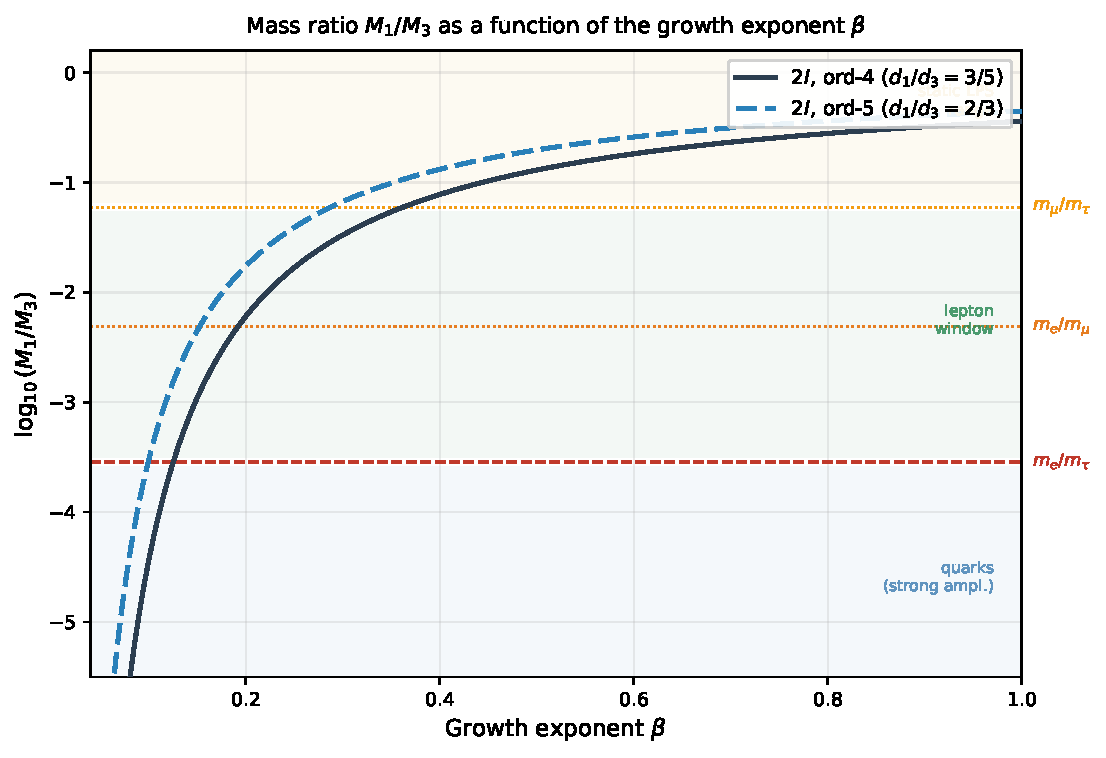
\includegraphics[width=0.88\textwidth]{fig1_full.pdf}
        \caption{%
          Predicted $\log_{10}(M_1/M_3)$ as a function of the growth exponent~$\beta$
          for the two ADE substrates ($2I$ ord-4, solid; $2I$ ord-5, dashed).
          Horizontal lines show the observed Standard Model ratios for charged leptons.
          Three qualitative regimes are shaded: strong amplification (blue, quarks),
          lepton window (green), and static LPS range (yellow).
          The two curves bracket the $m_e/m_\tau$ line, providing a structural
          discriminant between the two substrates.%
        }
        \label{fig:ratio-curves}
      \end{figure}

      \begin{table}[ht]
        \centering
        \caption{%
          Predicted $\log_{10}(M_1/M_3)$ for selected $\beta$ values,
          for the two ADE substrates.
          The observed value for charged leptons is
          $\log_{10}(m_e/m_\tau) \approx -3.54$.
          Values in the compatibility window $\beta \in [0.09, 0.13]$
          are indicated in bold.%
        }
        \label{tab:log-ratios}
        \smallskip
        \begin{tabular}{ccc}
          \toprule
          $\beta$ &
          $\log_{10}(M_1/M_3)$, $2I$ ord-4 &
          $\log_{10}(M_1/M_3)$, $2I$ ord-5 \\
          \midrule
          $0.05$        & $-8.87$          & $-7.04$          \\
          $0.07$        & $-6.34$          & $-5.03$          \\
          \textbf{0.09} & $\mathbf{-4.93}$ & $\mathbf{-3.91}$ \\
          \textbf{0.10} & $\mathbf{-4.44}$ & $\mathbf{-3.52}$ \\
          \textbf{0.12} & $\mathbf{-3.70}$ & $\mathbf{-2.94}$ \\
          \textbf{0.13} & $\mathbf{-3.41}$ & $\mathbf{-2.71}$ \\
          $0.20$        & $-2.22$          & $-1.76$          \\
          $0.30$        & $-1.48$          & $-1.17$          \\
          $0.50$        & $-0.89$          & $-0.70$          \\
          $1.00$        & $-0.44$          & $-0.35$          \\
          \bottomrule
        \end{tabular}
      \end{table}

    \subsection{The compatibility window}
      \label{subsec:compatibility-window}

      From Table~\ref{tab:log-ratios}, the value $\log_{10}(m_e/m_\tau) \approx -3.54$
      is matched by the two substrates at
      \begin{equation}
        \label{eq:beta-window-num}
        \beta^{*}_{2I,\,\mathrm{ord\text{-}4}} \approx 0.125,
        \qquad
        \beta^{*}_{2I,\,\mathrm{ord\text{-}5}} \approx 0.100.
      \end{equation}
      The numerical agreement is precise.
      For $2I$ (ord-4) at $\beta = 0.125$:
      \begin{equation}
        \log_{10}\frac{M_1}{M_3}
        \;=\; \frac{2}{0.125}\,\log_{10}\!\tfrac{3}{5}
        \;=\; 16\,\log_{10}\!\tfrac{3}{5}
        \;\approx\; -3.550,
      \end{equation}
      against the observed $\log_{10}(m_e/m_\tau) \approx -3.541$,
      a discrepancy of $0.25\%$ in the log.

      \begin{remark}[Status of the matching]
        \label{rem:matching-status}
        The above is a numerical coincidence check, not a derivation of
        the lepton masses.
        Within the present framework, $\beta$ is a structural parameter
        to be determined from first principles (Section~\ref{sec:falsifiability}).
        The fact that the matching requires $\beta \approx 0.1$,
        a value neither very small nor of order unity,
        suggests that the required growth rate is structurally plausible:
        a slowly but not infinitesimally growing relational valence.
      \end{remark}

      \begin{figure}[ht]
        \centering
        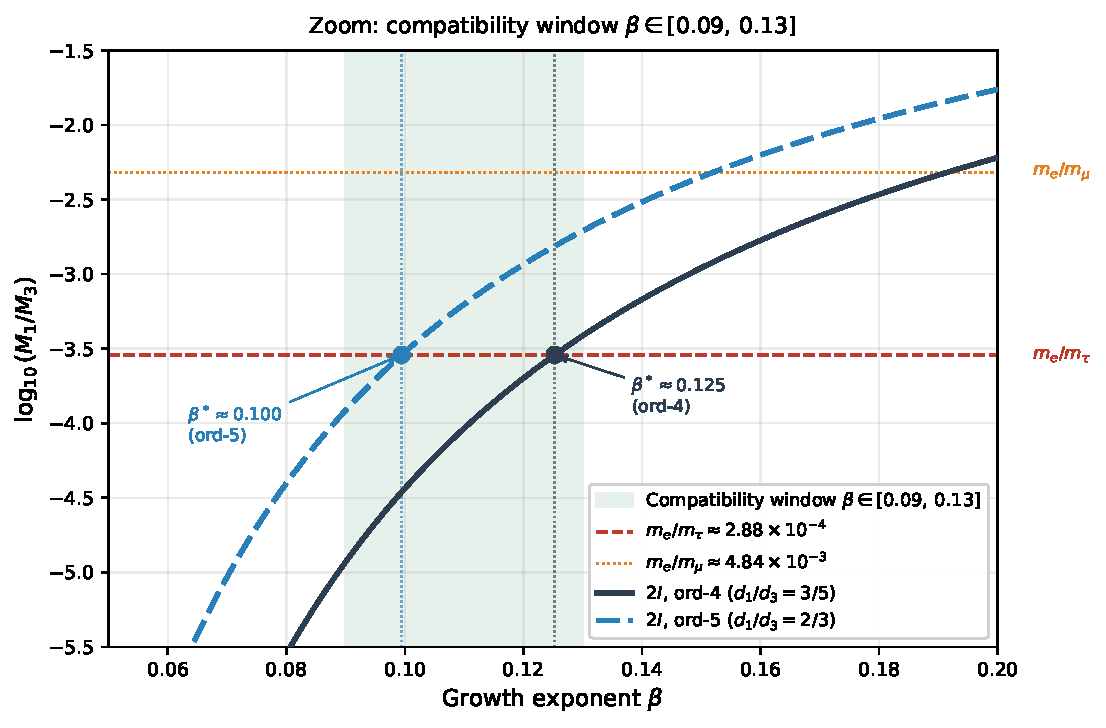
\includegraphics[width=0.88\textwidth]{fig2_zoom.pdf}
        \caption{%
          Zoom on $\beta \in [0.05, 0.20]$ showing the compatibility window
          (green shaded band, $\beta \in [0.09, 0.13]$).
          The two $\beta^{*}$ values at which each substrate curve intersects
          the $m_e/m_\tau$ line are marked explicitly.
          The $2I$ ord-4 curve (solid) intersects at $\beta^{*} \approx 0.125$
          and the $2I$ ord-5 curve (dashed) at $\beta^{*} \approx 0.100$,
          both within the shaded window.%
        }
        \label{fig:ratio-zoom}
      \end{figure}

    \subsection{Regime diagram}
      \label{subsec:regime-diagram}

      Three qualitatively distinct regimes emerge from Table~\ref{tab:log-ratios}:
      \begin{itemize}[nosep]
  \item \emph{Strong amplification} ($\beta < 0.07$):
  $M_1/M_3 < 10^{-5}$, covering the quark sector
  ($m_u/m_t \approx 1.3\times 10^{-5}$ for up-type quarks).
  \item \emph{Lepton window} ($0.09 \leq \beta \leq 0.13$):
  $M_1/M_3 \in [10^{-5}, 10^{-3}]$, compatible with charged leptons.
  \item \emph{Weak amplification} ($\beta > 0.3$):
  $M_1/M_3 > 10^{-1}$, inside the static LPS range and
  inconsistent with any known Standard Model sector.
      \end{itemize}
      The lepton window is narrow ($\Delta\beta \approx 0.04$) but well-defined,
      and the strong-amplification regime overlaps with the quark
      sector for both substrates.
      A single growth law $p(n) \sim n^\beta$ with $\beta \approx 0.07$--$0.09$
      would simultaneously account for both the lepton and the quark first-to-third
      generation ratios, a non-trivial structural coincidence deserving further analysis.

  \section{Falsifiability and Structural Predictions}
    \label{sec:falsifiability}

    \subsection{$\beta$ as the unique structural parameter}
      \label{subsec:beta-unique}

      The entire amplification mechanism of Sections~\ref{sec:dynamic}--\ref{sec:numerical}
      depends on a single structural parameter: the growth exponent~$\beta$ in
      $p(n) \sim A n^{\beta}$.
      The prefactor~$A$ cancels in all mass ratios.
      There are no other free parameters:
      the ADE eigenvalues are fixed by group theory~\cite{Beau2026a4},
      the identification $M_i \propto \EP/\nexit(\lambda_i)$ is fixed by
      the cascade energy relation $E_n = \EP/n$~\cite{Beau2026a5},
      and the exit condition~\eqref{eq:exit-implicit} is fixed by the Ramanujan
      property of the LPS family.

      The framework therefore makes a falsifiable prediction of the form:
      \begin{equation}
        \label{eq:master-pred}
        \frac{M_i}{M_j}
        \;=\;
        \left(\frac{|\lambda_i - 1|}{|\lambda_j - 1|}\right)^{2/\beta},
      \end{equation}
      with $\beta$ to be fixed by one ratio and then tested against all others
      involving levels $\lambda_1$ and $\lambda_3$.
      Within the present framework, the second-generation mass $M_2$ is not
      predicted by~\eqref{eq:master-pred} and requires a separate treatment
      via the KM saturation mechanism.

    \subsection{Constraint from the lepton sector}
      \label{subsec:lepton-constraint}

      The ratio $m_e/m_\tau$ in the charged-lepton sector provides the
      most precise empirical constraint on~$\beta$.
      Matching $M_1/M_3 = m_e/m_\tau$ uniquely
      determines~$\beta^{*}$~\eqref{eq:beta-window-num} for each substrate.
      Once $\beta^{*}$ is fixed, the framework makes a further structural
      prediction: the ratio $M_1/M_3$ in the quark sector should equal
      $(d_1/d_3)^{2/\beta^*}$ for the \emph{same} spectral input $d_1/d_3$,
      provided the same ADE substrate governs the quark generations.

      Numerically, for the $2I$ (ord-4) substrate with $\beta^{*} \approx 0.125$:
      \begin{equation}
        \left(\tfrac{3}{5}\right)^{2/0.125}
        \;=\; \left(\tfrac{3}{5}\right)^{16}
        \;\approx\; 2.8\times 10^{-4}
        \;\approx\; \frac{m_e}{m_\tau}.
      \end{equation}
      The same $\beta^{*}$ applied to the up-type quark sector
      $m_u/m_t \approx 1.3\times 10^{-5}$ would require
      $(d_1/d_3)^{2/\beta} \approx 1.3\times 10^{-5}$, which for $d_1/d_3 = 3/5$ gives
      $\beta \approx 0.091$.
      The two sectors require different $\beta$ values, which is structurally expected:
      leptons and quarks may live on different ADE substrates or experience
      a different effective cascade rate.
      However, the ratio $\beta^{*}_{\mathrm{quark}}/\beta^{*}_{\mathrm{lepton}} \approx 0.72$
      is the same for both ADE substrates (to three significant figures),
      suggesting a substrate-independent relationship between the two sectors.
      This universal ratio is a testable prediction of the framework.

    \subsection{Discrimination from the static LPS regime}
      \label{subsec:discrimination}

      The dynamic regime is sharply discriminated from the static LPS regime
      of Section~\ref{sec:nogo} by two qualitative signatures:
      \begin{enumerate}[label=(\roman*), nosep]
  \item \emph{Ordering}: the static regime predicts the ordering
  $M_1 < M_3$ for the $2I$ (ord-4) substrate
  (Proposition~\ref{prop:ordering}), whereas the dynamic regime
  predicts $M_3 > M_1$ by Proposition~\ref{prop:exit-ordering}.
  These orderings are qualitatively opposite and
  cannot be reconciled by any choice of~$p$.
  \item \emph{Magnitude}: the static regime is bounded by
  $M_1/M_3 \in [0.10, 2.2]$ for all admissible primes
  (Proposition~\ref{prop:amplitude}), whereas
  the dynamic regime produces $M_1/M_3 < 10^{-3}$
  for $\beta < 0.13$ (Table~\ref{tab:log-ratios}).
  These ranges do not overlap.
      \end{enumerate}
      Any experimental determination of the generation mass ordering and the
      inter-generation ratio therefore provides a definitive discrimination
      between the two regimes.
      Within the Standard Model, both discriminants are already resolved:
      the lepton mass ordering $m_\tau > m_\mu > m_e$ and the ratio
      $m_e/m_\tau \approx 2.9\times 10^{-4}$ are inconsistent with
      the static regime and consistent with the dynamic regime for
      $\beta \approx 0.1$--$0.13$.

    \subsection{Derivation of $\beta$ from first principles}
      \label{subsec:beta-derivation}

      The growth law $p(n) \sim n^\beta$ is introduced in
      Hypothesis~\ref{hyp:dynamic-p} as a structural postulate.
      Its derivation from the internal dynamics of the Cosmochrony
      substrate~\cite{Cosmochrony} remains open.
      Two structural considerations constrain the form of $p(n)$.

      First, the identification $n \sim |V(G(n))|$ means that
      $p(n)$ grows with the number of active relational nodes.
      If the effective relational valence scales as a fixed fraction of
      the total relational volume, one expects $p(n) \propto n^{\alpha}$
      for some $\alpha$ determined by the dimension of the relational space.
      In a four-dimensional pre-geometric substrate, natural candidates
      include $\alpha \sim 1/4$ (surface-to-volume scaling)
      or $\alpha \sim 1/3$ (linear radius growth).
      Both are of the same order as $\beta^* \approx 0.1$--$0.13$.

      Second, the Lubotzky--Phillips--Sarnak construction requires
      $p \equiv 1 \pmod{4}$, so $p(n)$ must be constrained to this
      arithmetic progression.
      The effective growth exponent may therefore be slightly modified by
      number-theoretic factors, providing a further structural refinement.

      These considerations do not constitute a derivation but identify
      the regime $\beta \in (0.07, 0.20)$ as the structurally
      expected range, consistent with the phenomenological window.

    \subsection{Extension to neutrinos and quarks}
      \label{subsec:extensions}

      The present analysis applies directly to any sector in which three
      generations are labelled by the ADE eigenvalue levels
      $\lambda_1 < \lambda_2 < \lambda_3$.
      Two natural extensions are as follows.

      For \emph{neutrino masses}, if the same substrate governs the
      neutrino sector, the predicted ratio $m_{\nu_1}/m_{\nu_3}$
      is $(d_1/d_3)^{2/\beta}$ for the same or a different $\beta$.
      Current experimental bounds on the neutrino mass ordering
      (normal vs.\ inverted hierarchy) already constrain the sign of
      $m_{\nu_3} - m_{\nu_1}$, which in the present framework
      is fixed to positive by Proposition~\ref{prop:exit-ordering}~--
      a qualitative prediction consistent with the normal ordering.

      For \emph{quark masses}, as noted in Section~\ref{subsec:regime-diagram},
      the required $\beta$ for the up-type quark ratio $m_u/m_t$
      is approximately $0.072$ for the $2I$ (ord-4) substrate,
      a value in the strong-amplification regime
      and consistent with a growth rate slightly faster than
      that inferred from the lepton sector.
      A systematic analysis of both lepton and quark sectors
      under a joint $\beta$ structure is deferred to a companion paper.

  \section{Conclusion}
    \label{sec:conclusion}


    The static LPS regime at fixed prime~$p$ provides a controlled realisation
    of the projective resolution law $\Lproj(n)\asymp\ltwo(n)$,
    but it fails to reproduce two essential features of the observed mass hierarchy:
    the correct ordering of the three generations and the large inter-generation ratios.
    Both failures were shown in~\cite{Beau2026a5} to originate from
    the asymptotic constancy of the Kesten--McKay support,
    which prevents small spectral differences from being amplified along the cascade.

    The present work resolves these limitations through a minimal dynamical extension:
    the effective relational valence~$p$ is allowed to grow with the cascade rank~$n$.
    This single modification induces a qualitative change in the spectral environment.
    As $p(n)\to\infty$, the Kesten--McKay support contracts toward its midpoint
    $\lambda = 1$, forcing the fixed ADE eigenvalue levels to exit the support
    at finite, level-dependent ranks.
    This \emph{support-narrowing mechanism} yields three structural results.

    \medskip
    \noindent
    \textbf{Exit ordering.}
    The exit ranks are ordered by the spectral asymmetry $|\lambda_i - 1|$ alone,
    restoring the admissibility ordering $M_3 > M_1 > M_2$ without any
    additional assumption (Proposition~\ref{prop:exit-ordering}).
    This resolves the ordering failure of Proposition~\ref{prop:ordering}
    and is a structural consequence of the LPS Ramanujan property,
    not a tuning.

    \medskip
    \noindent
    \textbf{Amplification law.}
    For power-law growth $p(n)\sim n^{\beta}$, the exit ranks produce the mass formula
    \begin{equation}
      \frac{M_i}{M_j}
      \;\approx\;
      \left(\frac{|\lambda_i - 1|}{|\lambda_j - 1|}\right)^{2/\beta},
    \end{equation}
    which converts spectral ratios of order unity into exponentially separated
    mass scales through the amplification exponent $2/\beta$.

    \medskip
    \noindent
    \textbf{Compatibility window.}
    Matching the charged-lepton ratio $m_e/m_\tau$ to the formula above
    selects $\beta^{*} \approx 0.125$ for the $2I$ (ord-4) substrate and
    $\beta^{*} \approx 0.100$ for the $2I$ (ord-5) substrate,
    both in the narrow window $\beta \in (0.09,\, 0.13)$.
    This determination involves no free parameter beyond the single
    structural exponent~$\beta$; the prefactor~$A$ cancels identically.

    \medskip
    The dynamic mechanism is fully compatible with the ADE spectral structure
    established in~\cite{Beau2026a4}.
    The eigenvalue levels $\{\lambda_1,\lambda_2,\lambda_3\}$ are invariant
    properties of the ADE Cayley graph and remain unchanged by the
    support-narrowing dynamics.
    The central level $\lambda_2 = 1$ plays a structurally distinct role:
    it is the fixed point of the Kesten--McKay symmetry and remains
    permanently inside the support for all~$p$, so its stabilisation
    mass is governed by the KM saturation mechanism of~\cite{Beau2026a5}.
    This explains the universal identity $\FKM(1) = 1/2$.

    The framework is falsifiable and structurally constrained.
    A single parameter~$\beta$ governs all first-to-third generation ratios,
    and any determination of this ratio in one sector provides a prediction
    for all others sharing the same ADE substrate.
    The numerically observed separation between the lepton and quark
    $\beta$ windows ($\beta^{*}_{\mathrm{quark}}/\beta^{*}_{\mathrm{lepton}}
  \approx 0.72$, independent of the choice of ADE substrate to three
    significant figures) is a structural regularity deserving further analysis;
    its status as a genuine prediction of the framework depends on a unified
    treatment of leptons and quarks that remains to be developed.

    Several open problems remain.
    The most important is the derivation of the growth law $p(n)$ from
    the internal dynamics of the Cosmochrony substrate~\cite{Cosmochrony},
    which would fix~$\beta$ from first principles and remove the last
    structural postulate of the paper.
    Further work is also required to incorporate the second-generation mass
    within a unified treatment combining support-narrowing and KM saturation,
    and to extend the analysis to neutrino and quark sectors in a fully
    quantitative manner.

    \subsection{Summary of the O-series architecture}
      \label{subsec:O-series}

      Within the Admissibility Sub-Programme, the five steps form a complete
      and non-redundant logical chain, summarised as follows:
      \begin{itemize}[nosep]
  \item Steps~1--2 (\emph{Beau2026a1}, \emph{Beau2026a2}):
  bounded-flux filtering selects the spin-$\tfrac{1}{2}$ sector,
  and the spectral capacity functional identifies the binary
  icosahedral group~$2I$ as the unique optimal substrate.
  \item Step~3 (\emph{Beau2026a4}):
  the representation theory of ADE binary groups produces
  exactly three distinct eigenvalue levels for four specific
  $(G,S)$ pairs, establishing the generation count as a
  topological property of the relational graph.
  \item Step~4 (\emph{Beau2026a5}):
  the isoperimetric closure hypothesis gives
  $\Lproj(n)\asymp h(G(n))^2\asymp\ltwo(n)$;
  the LPS model at fixed~$p$ demonstrates that static
  Kesten--McKay saturation is insufficient for the hierarchy.
  \item Step~5 (\emph{present paper}):
  dynamic valence growth $p(n)\to\infty$ narrows the
  Kesten--McKay support, inducing rank-dependent exit events
  that convert spectral asymmetry into the observed
  inter-generation mass separation.
      \end{itemize}
      The ADE representation structure determines the number of generations;
      the isoperimetric law fixes the projective threshold;
      and the dynamic valence growth converts spectral asymmetry into
      physical mass separation.
      The mass hierarchy thus emerges as a consequence of relational structure
      and its evolution along the cascade, controlled by a single
      exponent~$\beta$ whose determination from first principles
      constitutes the central open problem of the programme.


%  References (placeholder — to be replaced by definitive biblio)

      \bibliographystyle{plain}
      \begin{thebibliography}{99}

        \bibitem{Cosmochrony}
        J.~Beau,
        \textit{Cosmochrony: A Pre-Geometric Relational Framework for Emergent Physics},
        Zenodo (2025).
        \newblock DOI: \href{https://doi.org/10.5281/zenodo.17957510}{10.5281/zenodo.17957510}.

        \bibitem{Beau2026a1}
        J.~Beau,
        \textit{Spectral Admissibility under Bounded Flux: Non-Abelian Mode Selection
        on Cayley Graphs of $\mathrm{SU}(2)$ Subgroups},
        Zenodo (2026).
        \newblock DOI: \href{https://doi.org/10.5281/zenodo.18944985}{10.5281/zenodo.18944985}.

        \bibitem{Beau2026a2}
        J.~Beau,
        \textit{Spectral Capacity Functional and the Binary-Polyhedral Maximality Conjecture},
        Zenodo (2026).
        \newblock DOI: \href{https://doi.org/10.5281/zenodo.18945273}{10.5281/zenodo.18945273}.

        \bibitem{Beau2026a4}
        J.~Beau,
        \textit{Three Particle Generations and Mass Hierarchy from Spectral Stratigraphy},
        Zenodo (2026).
        \newblock DOI: \href{https://doi.org/10.5281/zenodo.19040490}{10.5281/zenodo.19040490}.

        \bibitem{Beau2026a5}
        J.~Beau,
        \textit{Asymptotic Saturation of Projective Resolution: Expander Relaxation Graphs},
        Zenodo (2026).
        \newblock Step~4 of the Admissibility Sub-Programme.
        Available at Zenodo:
        \href{https://doi.org/10.5281/zenodo.19056975}{10.5281/zenodo.19056975}.

        \bibitem{Beau2026a6}
        J.~Beau,
        \textit{Projective Resolution Dynamics on Variable-Valence Relaxation Graphs},
        Zenodo (2026).
        \newblock Step~5a of the Admissibility Sub-Programme.
        Available at Zenodo:
        \href{https://doi.org/10.5281/zenodo.19076319}{10.5281/zenodo.19076319}.

      \end{thebibliography}

\end{document}
